% Don't touch this %%%%%%%%%%%%%%%%%%%%%%%%%%%%%%%%%%%%%%%%%%%
\documentclass[12pt]{article}
\usepackage{fullpage}
\usepackage[left=1in,top=1in,right=1in,bottom=1in,headheight=3ex,headsep=3ex]{geometry}
\usepackage{graphicx}
\usepackage{float}
\usepackage{array}


\newcommand{\blankline}{\quad\pagebreak[2]}
%%%%%%%%%%%%%%%%%%%%%%%%%%%%%%%%%%%%%%%%%%%%%%%%%%%%%%%%%%%%%%

% Modify Course title, instructor name, semester here %%%%%%%%

\title{Homework 4: Oscillations and waves II}
\author{PHY250 - Fall 2021}
\date{}

%%%%%%%%%%%%%%%%%%%%%%%%%%%%%%%%%%%%%%%%%%%%%%%%%%%%%%%%%%%%%%

% Don't touch this %%%%%%%%%%%%%%%%%%%%%%%%%%%%%%%%%%%%%%%%%%%
\usepackage[sc]{mathpazo}
%\linespread{1.05} % Palatino needs more leading (space between lines)
\usepackage[T1]{fontenc}
\usepackage[mmddyyyy]{datetime}% http://ctan.org/pkg/datetime
\usepackage{advdate}% http://ctan.org/pkg/advdate

\usepackage{setspace}

\newcommand{\HRule}{\rule{\linewidth}{0.5mm}}
\newdateformat{syldate}{\twodigit{\THEMONTH}/\twodigit{\THEDAY}}
\newsavebox{\MONDAY}\savebox{\MONDAY}{Mon}% Mon
\newcommand{\week}[1]{%
%  \cleardate{mydate}% Clear date
% \newdate{mydate}{\the\day}{\the\month}{\the\year}% Store date
  \paragraph*{\kern-2ex\quad #1, \syldate{\today} - \AdvanceDate[4]\syldate{\today}:}% Set heading  \quad #1
%  \setbox1=\hbox{\shortdayofweekname{\getdateday{mydate}}{\getdatemonth{mydate}}{\getdateyear{mydate}}}%
  \ifdim\wd1=\wd\MONDAY
    \AdvanceDate[7]
  \else
    \AdvanceDate[7]
  \fi%
}
%\usepackage{setspace}
\usepackage{multicol}
%\usepackage{indentfirst}
\usepackage{fancyhdr,lastpage}
\usepackage{url}
\pagestyle{fancy}
\usepackage{hyperref}
\usepackage{lastpage}
\usepackage{amsmath}
\usepackage{layout}

\lhead{}
\chead{}
%%%%%%%%%%%%%%%%%%%%%%%%%%%%%%%%%%%%%%%%%%%%%%%%%%%%%%%%%%%%%%

% Modify header here %%%%%%%%%%%%%%%%%%%%%%%%%%%%%%%%%%%%%%%%%
%\rhead{\footnotesize Text in header}

%%%%%%%%%%%%%%%%%%%%%%%%%%%%%%%%%%%%%%%%%%%%%%%%%%%%%%%%%%%%%%
% Don't touch this %%%%%%%%%%%%%%%%%%%%%%%%%%%%%%%%%%%%%%%%%%%
\lfoot{}
\cfoot{\small \thepage/\pageref*{LastPage}}
\rfoot{}

\usepackage{array, xcolor}
\usepackage{color,hyperref}
\definecolor{clemsonorange}{HTML}{EA6A20}
\hypersetup{colorlinks,breaklinks,linkcolor=clemsonorange,urlcolor=clemsonorange,anchorcolor=clemsonorange,citecolor=black}



\begin{document}


\maketitle

\textcolor{red}{Deadline: 23/19/2021}

\vspace{5mm}

\begin{spacing}{0.3}
    \noindent
    \HRule\\
    \HRule
\end{spacing}
\vspace{5mm}


% First Section %%%%%%%%%%%%%%%%%%%%%%%%%%%%%%%%%%%%%%%%%%%%


\newcounter{example}
\setcounter{example}{1}

\section*{Exercise \theexample }
Consider a simple pendulum of length $\ell=2$,  simulate its motion considering that it is not dumped. Do not consider small oscillations.\\
\vspace{3mm}
\\
Which numerical method is the best choice. What happens when you use the Euler Method? 

% First Section %%%%%%%%%%%%%%%%%%%%%%%%%%%%%%%%%%%%%%%%%%%%

\stepcounter{example}
\section*{Exercise \theexample }

Consider the motion of a mass attached to a spring ($m=1,k=1,x_0=1,v_0=0$), simulate the motion of the particle for the following cases:

\begin{enumerate}
    \item SHO motion.
    \item Damped motion with $b=0.1,b=1.1,b=b_{cri}$. 
    \item Compare the motion of both: plot the position, velocity and acceleration vs. time for all the cases.
    \item Now consider that there is also an external force with angular frequency $\omega$  that is acting on the system. Plot the the position vs. time for different frequencies $\omega$, make an animation.     
\end{enumerate}


% First Section %%%%%%%%%%%%%%%%%%%%%%%%%%%%%%%%%%%%%%%%%%%%


\stepcounter{example}
\section*{Exercise \theexample }
Calculate the first 40 terms of the Fourier expansion for a square wave (Fig.\ref{square}).
Make an animation in which you plot both, the function and the Fourier expansion.

\begin{figure}[h!]
  \begin{center}
    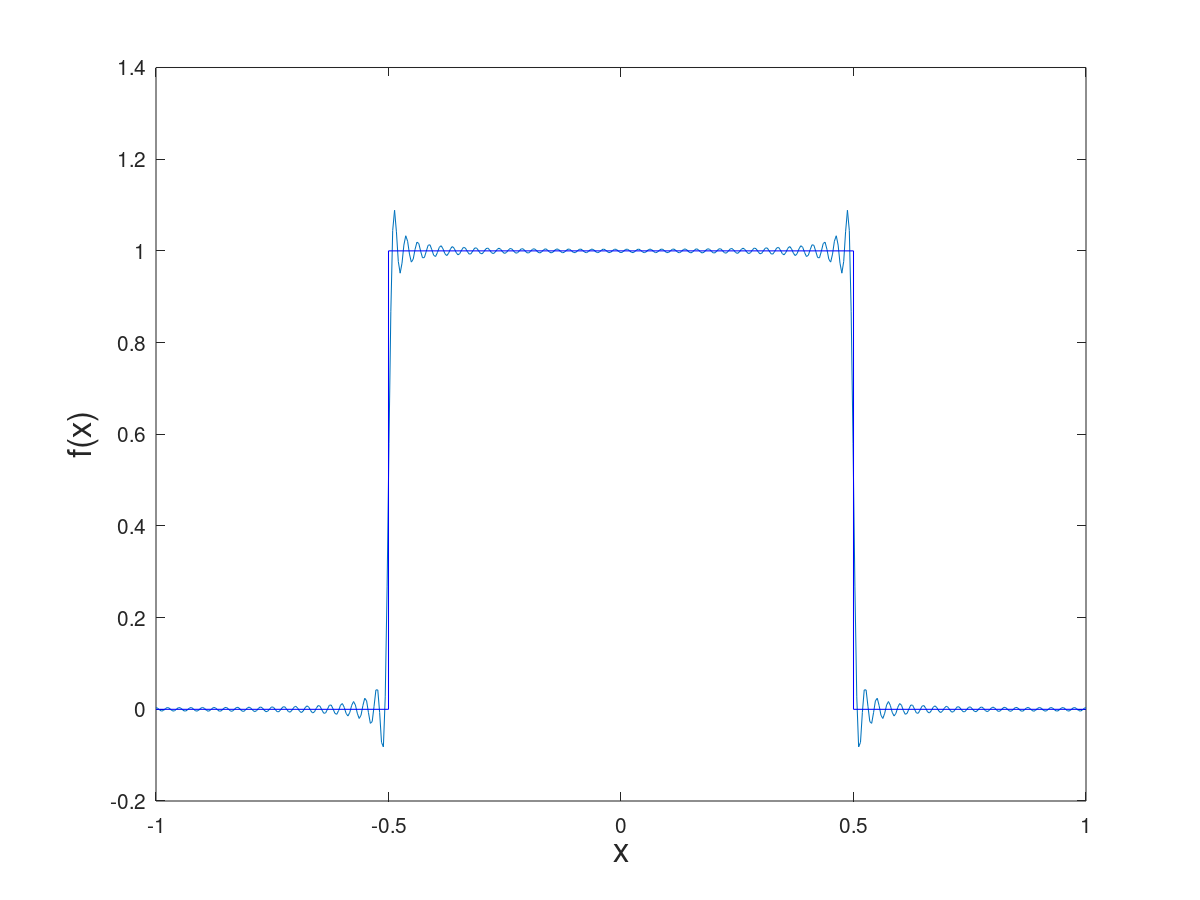
\includegraphics[height=4.in]{Solved/3/Animation4/00040.png}
    \caption{Square function + Fourier expansion.}  
    \label{square}
  \end{center}
\end{figure}



% % First Section %%%%%%%%%%%%%%%%%%%%%%%%%%%%%%%%%%%%%%%%%%%%
% \stepcounter{example}
% \section*{Exercise \theexample }

% Make an animation in which you represent traveling waves in 2D, consider that the medium is isotropic and you are:

% \begin{itemize}
%     \item close to the source.
%     \item far away from the source.
% \end{itemize}

% % First Section %%%%%%%%%%%%%%%%%%%%%%%%%%%%%%%%%%%%%%%%%%%%
% \stepcounter{example}
% \section*{Exercise \theexample }

% Now, make an animation considering that the medium in which the waves are traveling have limited dimensions. Consider a square of length $w,~\ell$. Make  animations for three different resonance modes.

% % First Section %%%%%%%%%%%%%%%%%%%%%%%%%%%%%%%%%%%%%%%%%%%%
% \stepcounter{example}
% \section*{Exercise \theexample }

% Simulate the pattern of interference between two equal sources separated by a distance $d$ in a 2d surface. 




\end{document}


